\begin{appendices}
%\addtocontents{toc}{\protect\setcounter{tocdepth}{0}}

\section{Grafana dashboard}
\label{dash1}

\begin{figure}[ht]
    \centering
    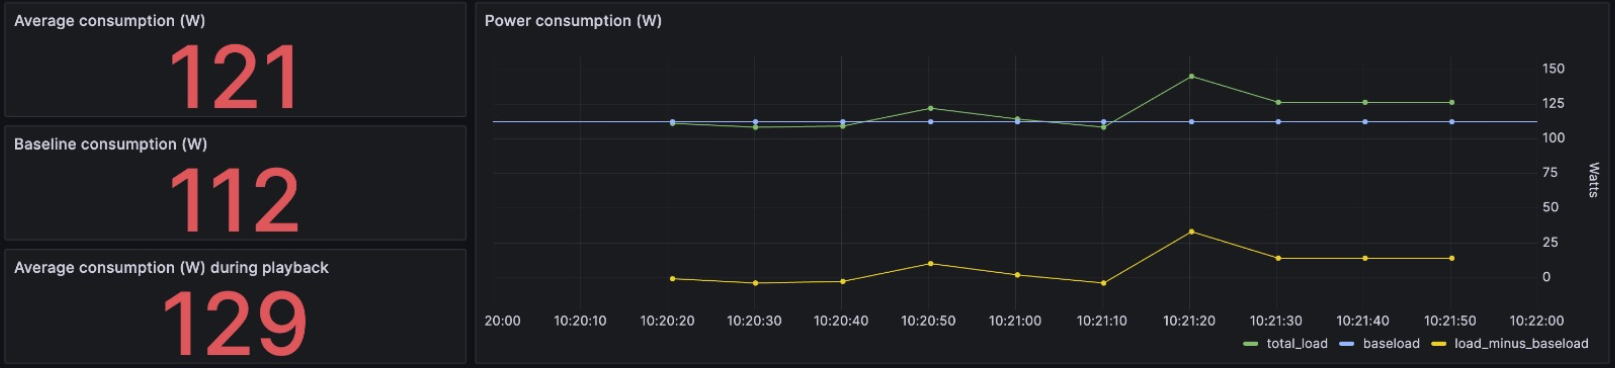
\includegraphics[width=1\linewidth]{assets/dashboard1.png}
    \caption{First graph of the Grafana dashboard}
    \label{fig:dash1}
\end{figure}

\begin{figure}[ht]
    \centering
    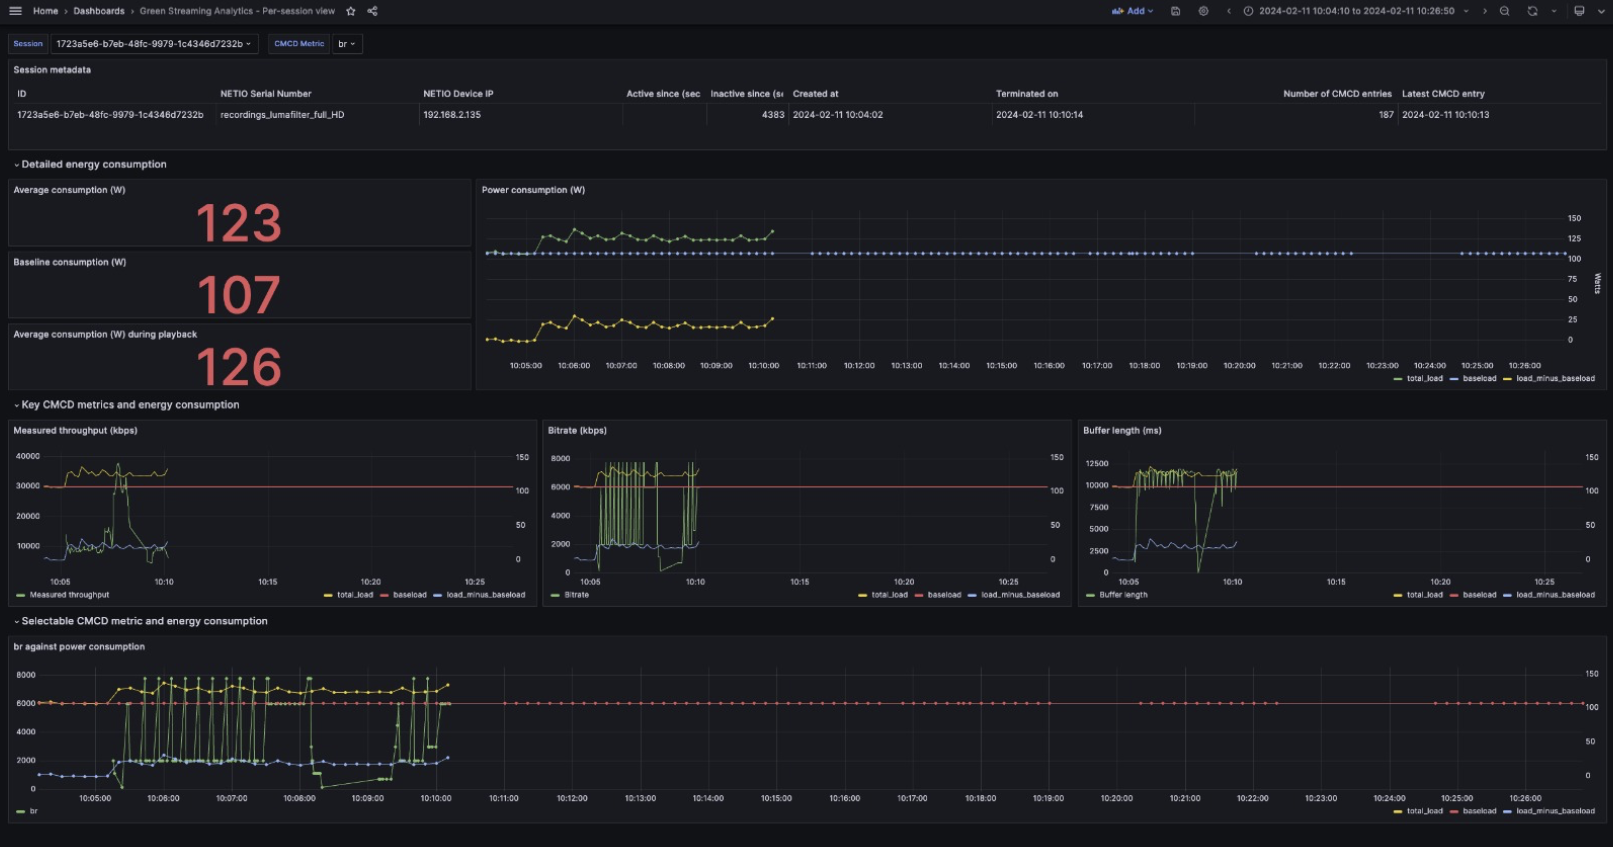
\includegraphics[width=1\linewidth]{assets/dashboard2.png}
    \caption{Second graph of the Grafana dashboard}
    \label{fig:dash2}
\end{figure}

\section{Player Application}

 \begin{figure}[ht]
     \centering
     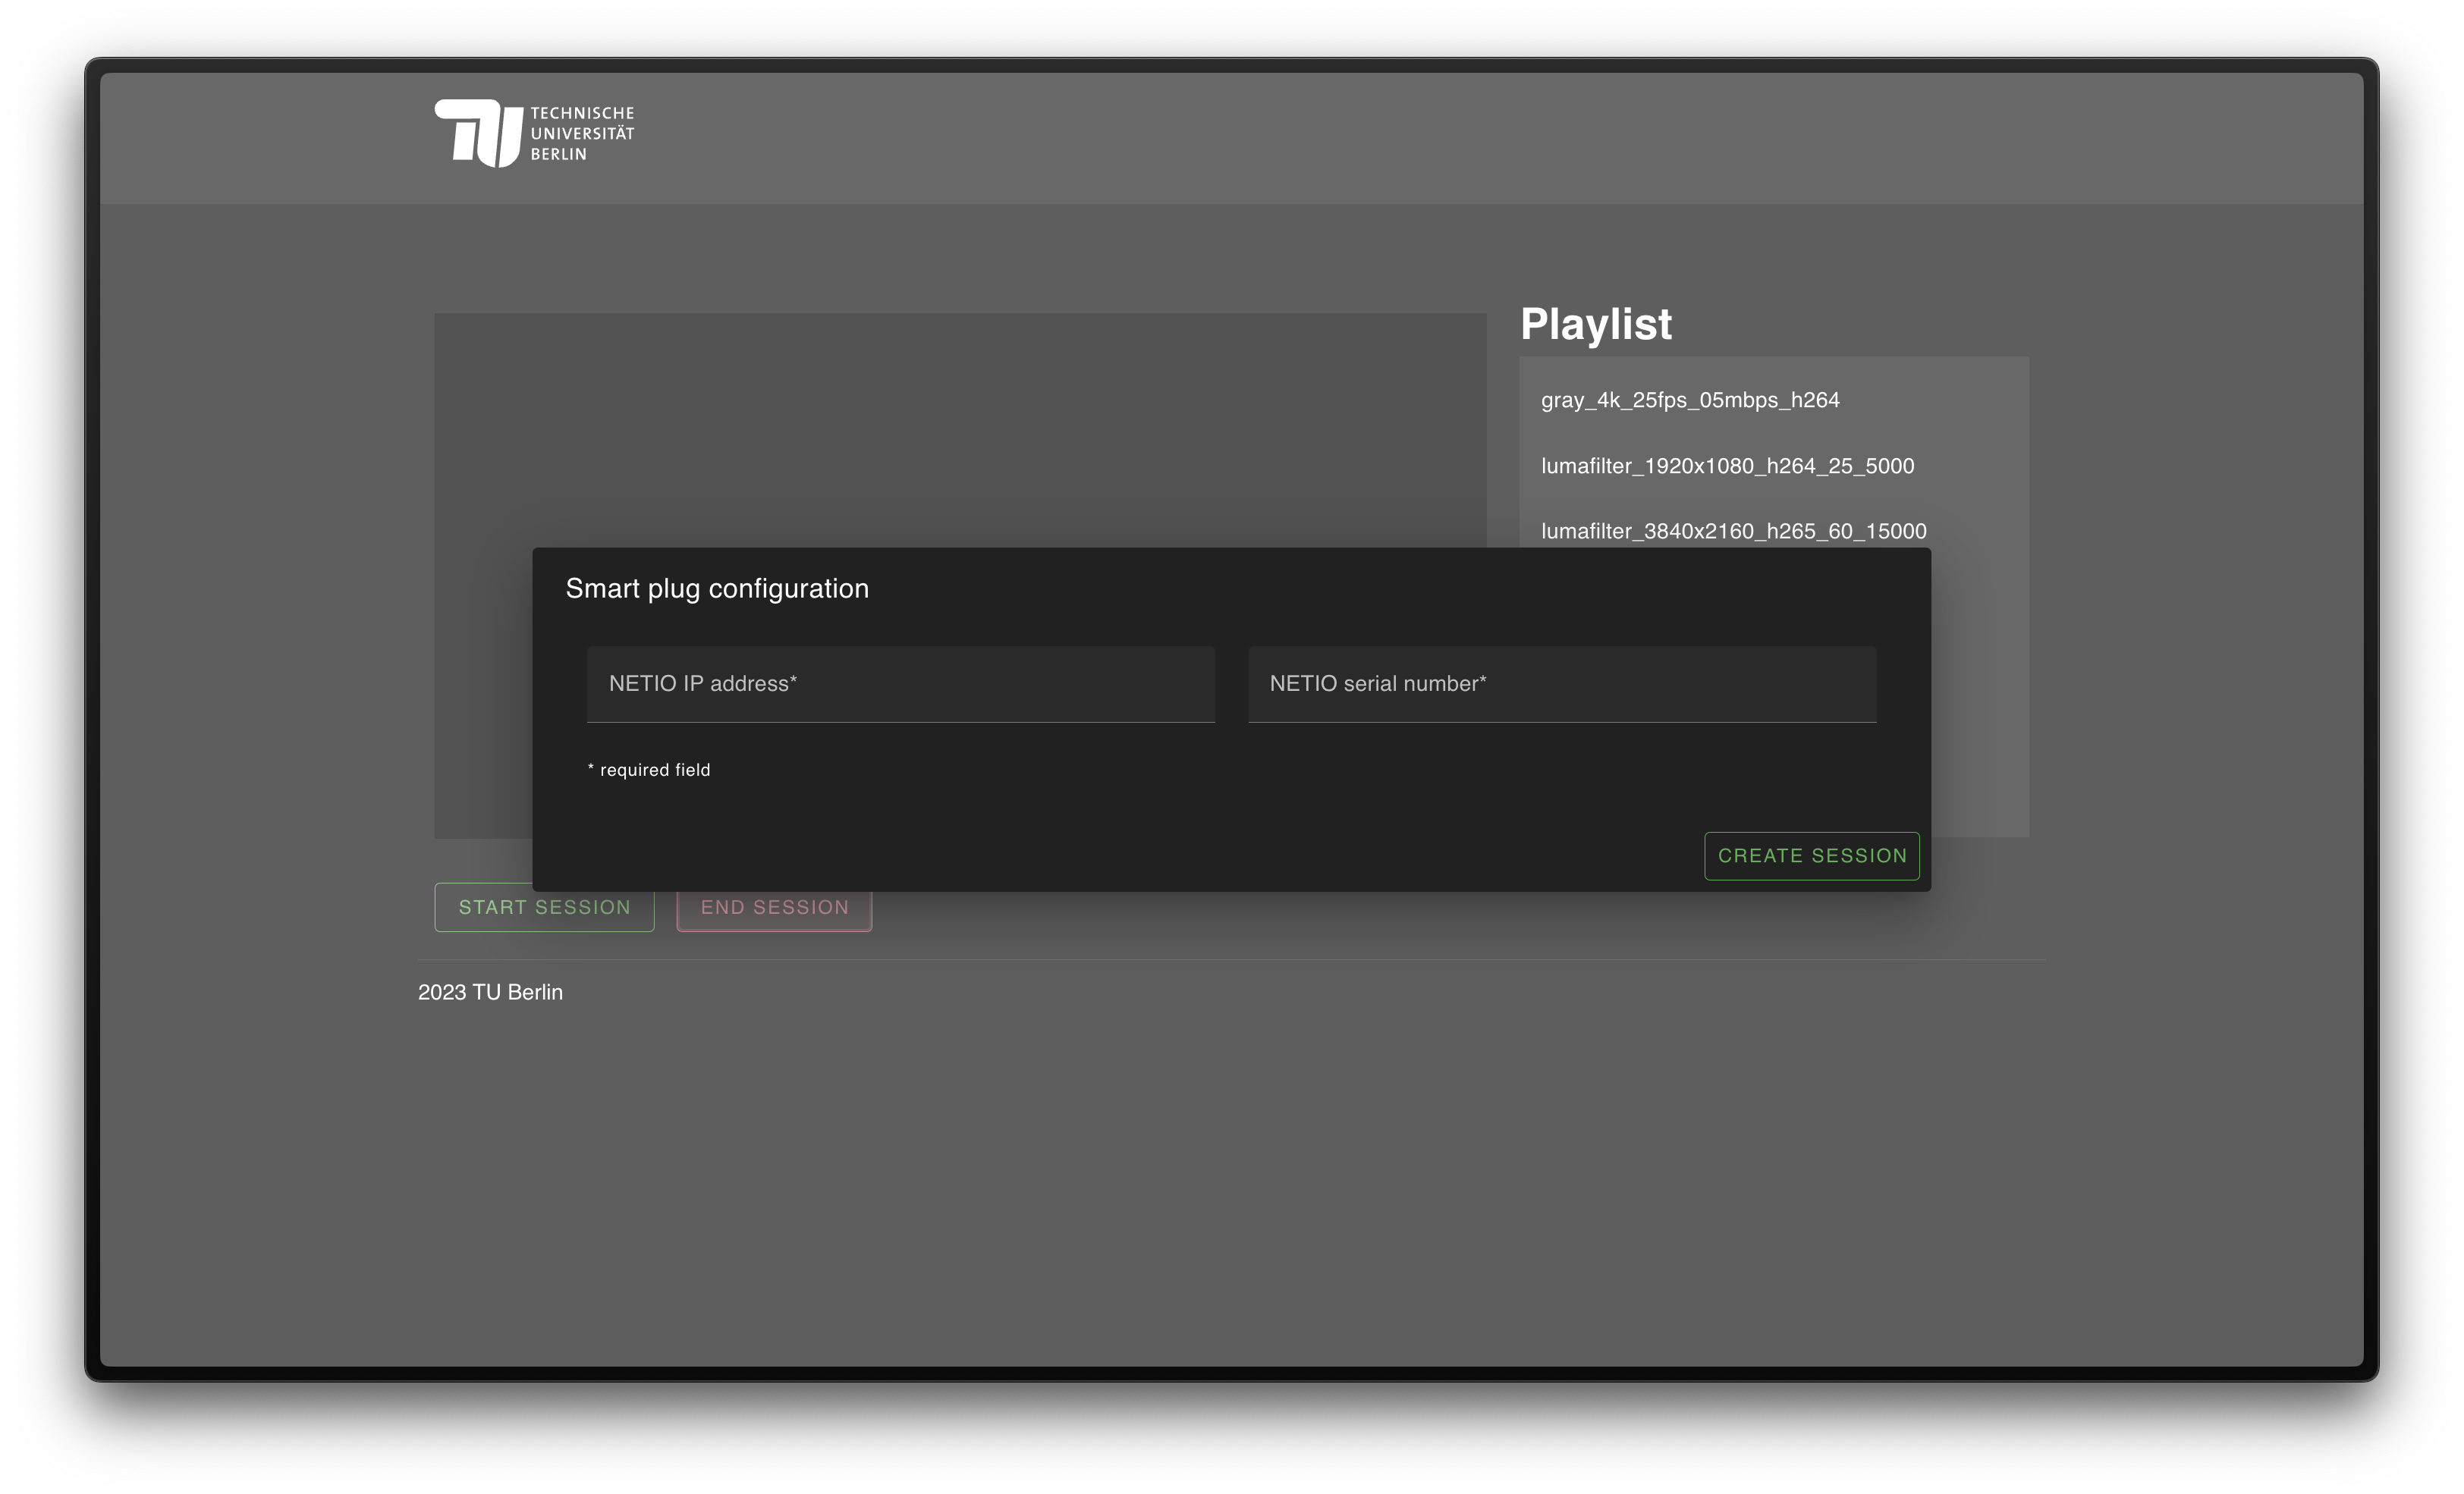
\includegraphics[width=0.8\linewidth]{assets/mediaplayer1.png}
     \caption{The landing page of the frontend application.}
     \label{fig:media_player1}
 \end{figure}

 \begin{figure}[ht]
     \centering
     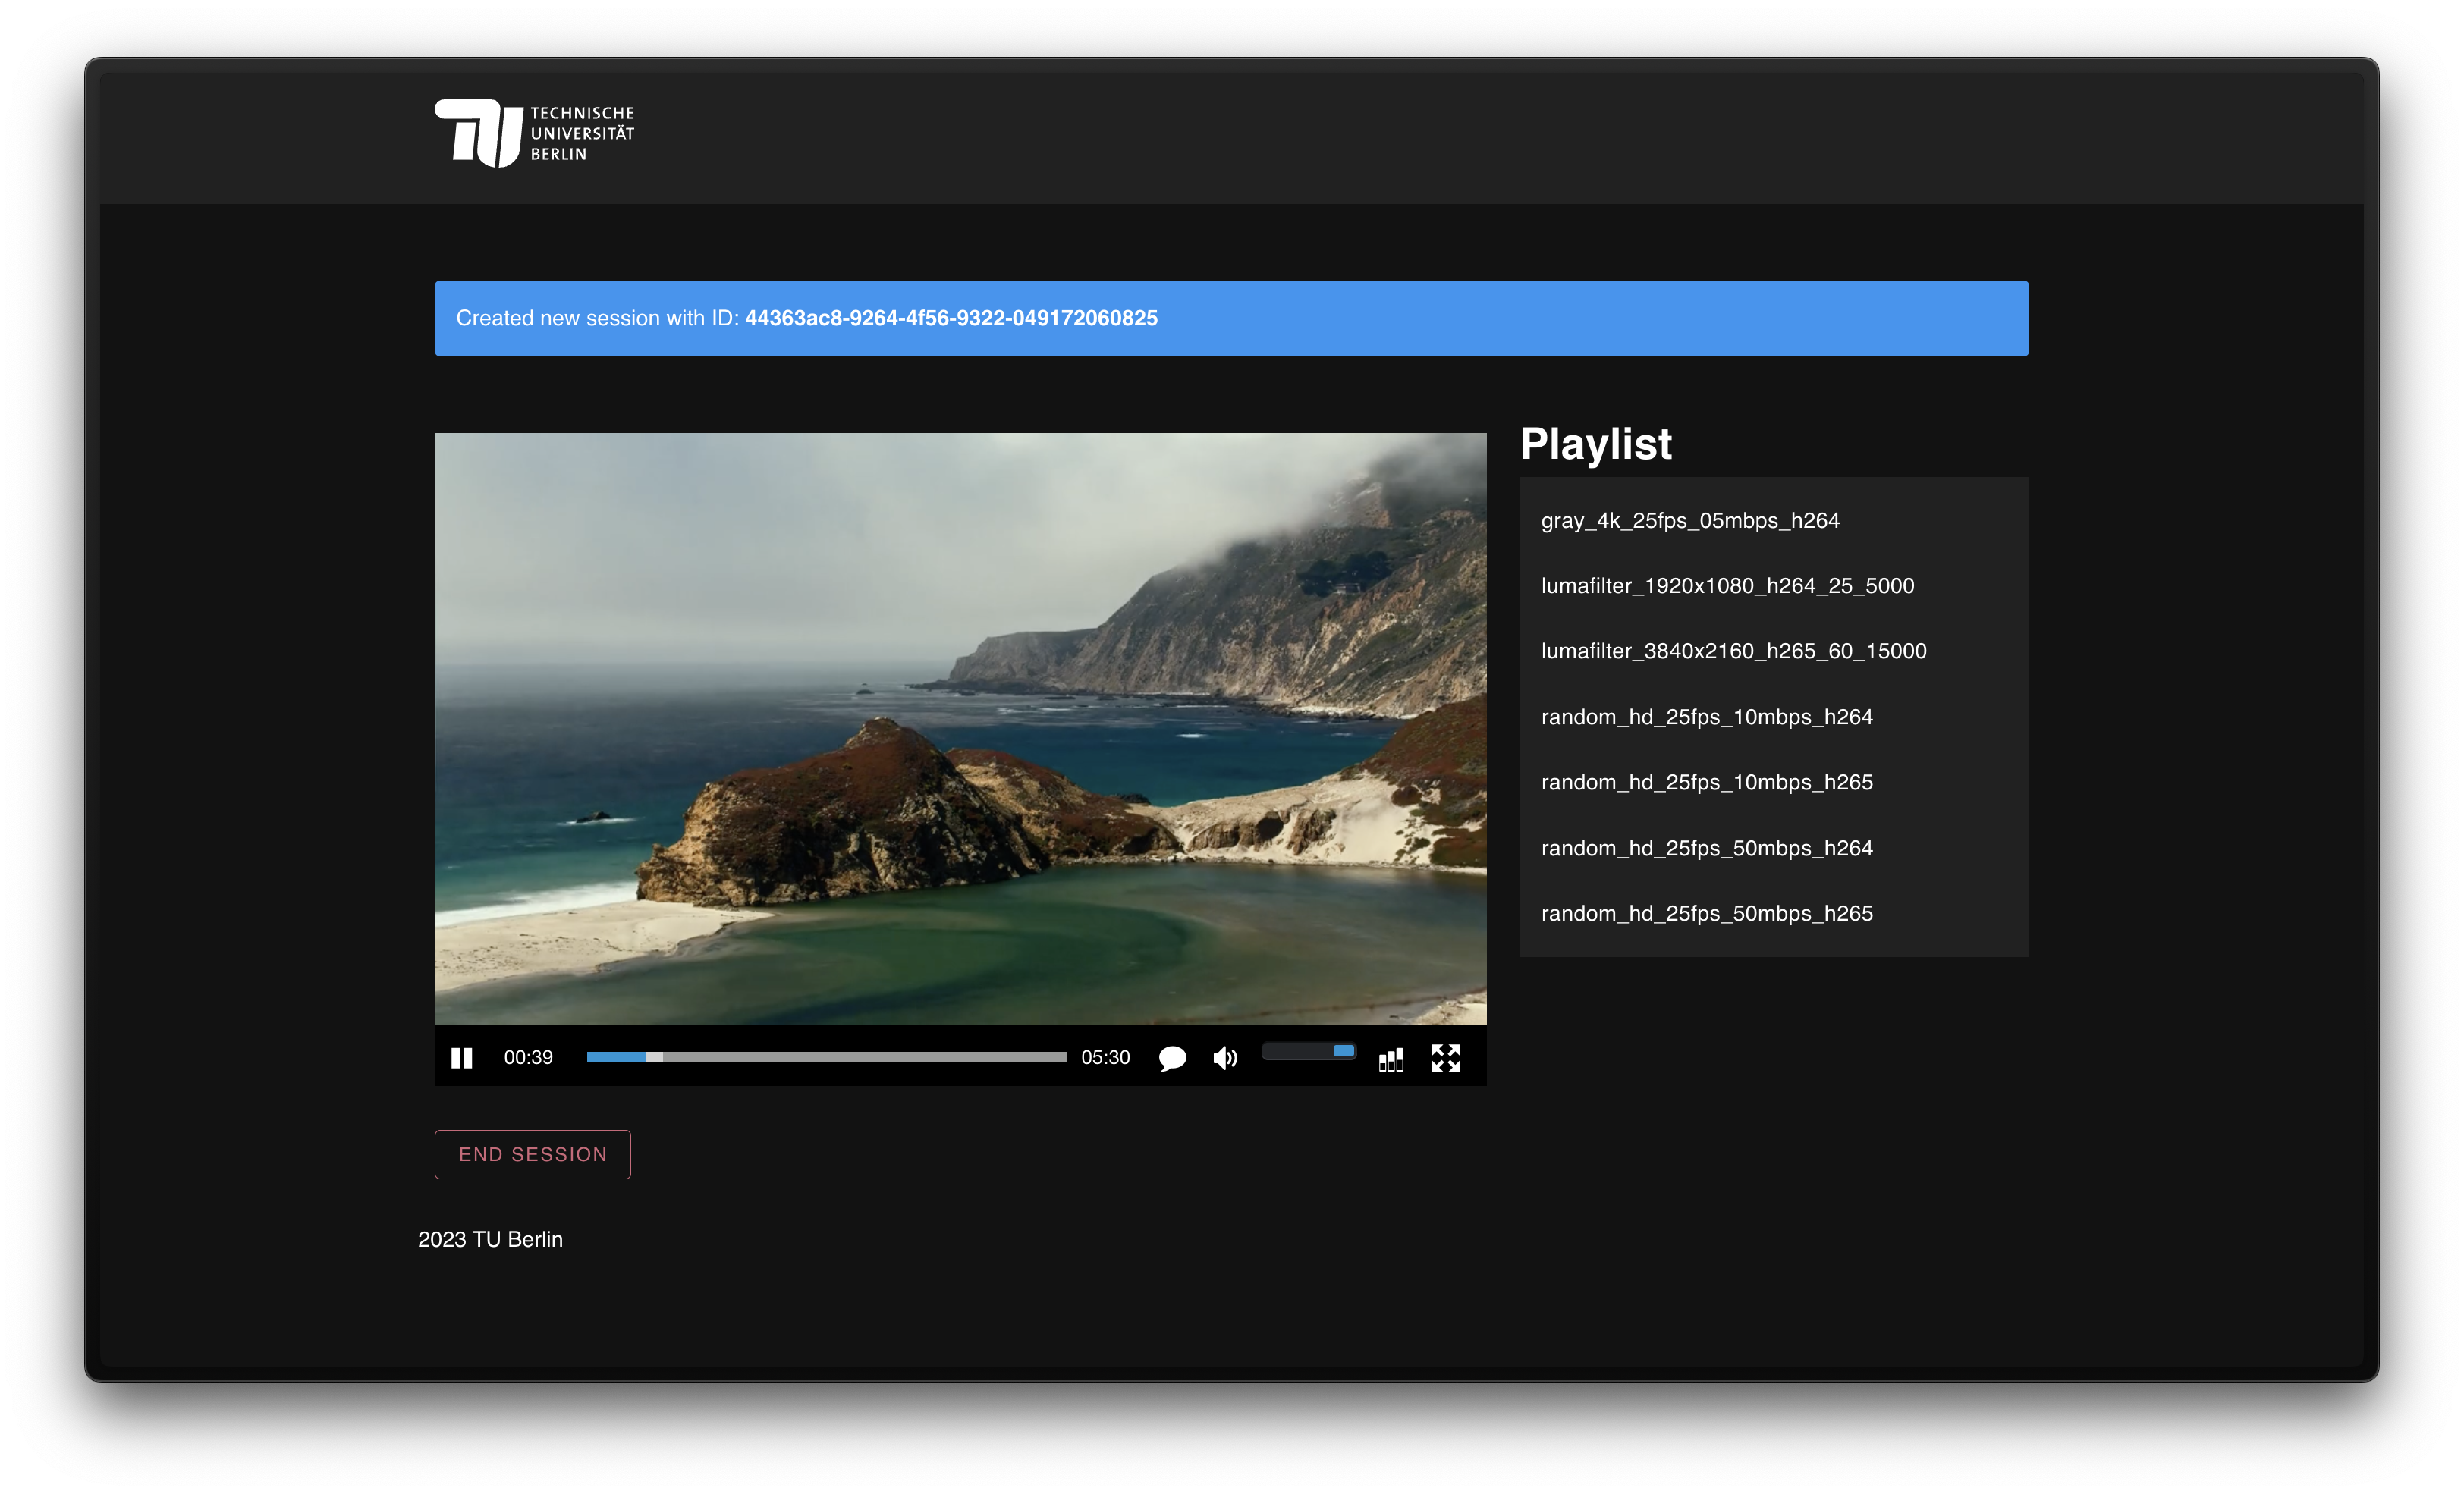
\includegraphics[width=0.8\linewidth]{assets/mediaplayer2.png}
     \caption{The frontend page of the application with the playlist and the player.}
     \label{fig:media_player2}
 \end{figure}

\section{Overall architecture}

 \begin{figure}[ht]
     \centering
     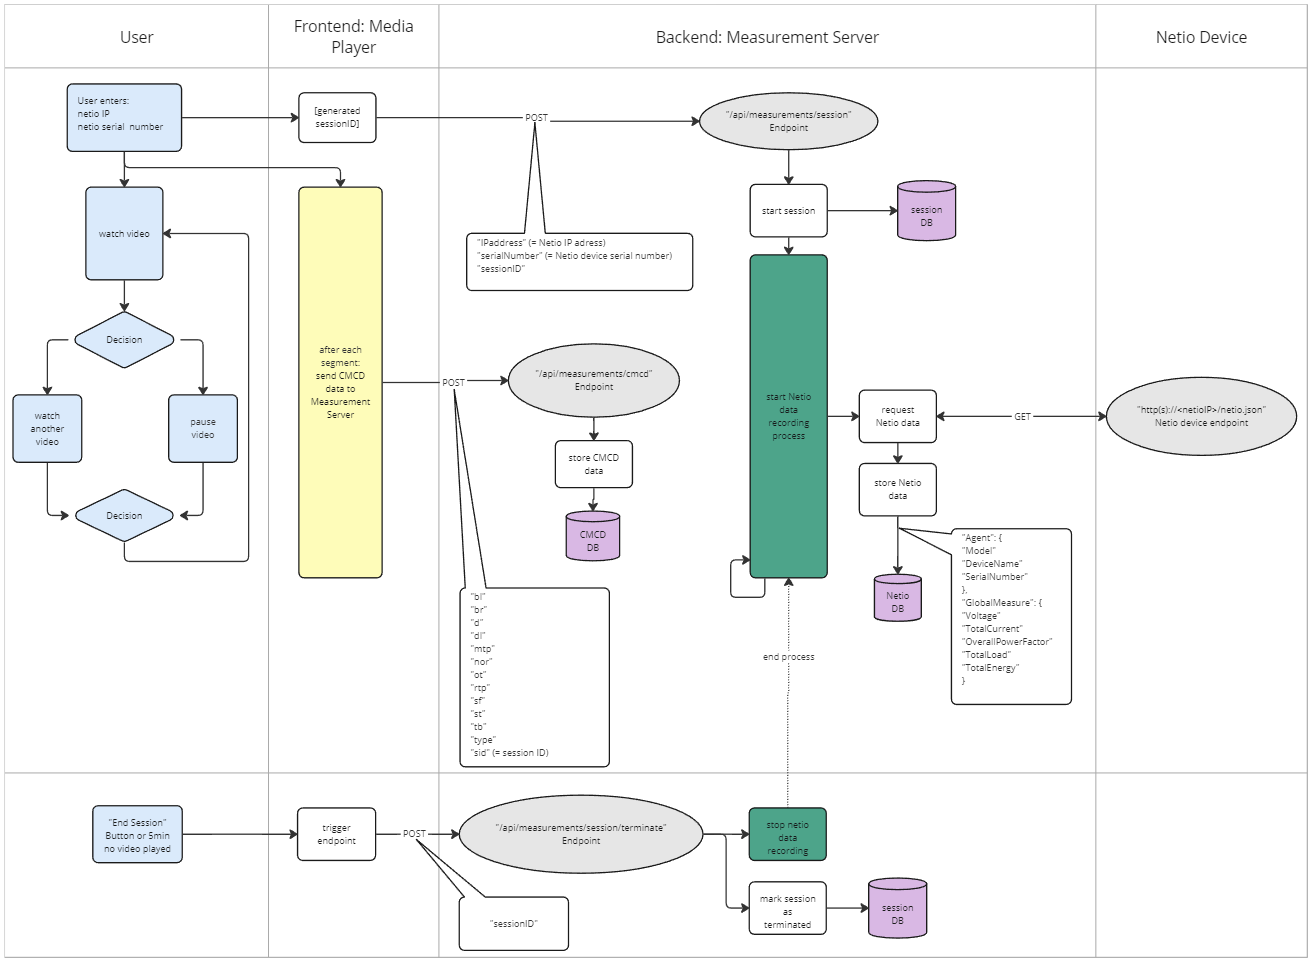
\includegraphics[width=1\linewidth]{assets/architecture_diagram.png}
     \caption{The overall architecture and internal process of the project.}
     \label{fig:project_architecture}
 \end{figure}


\section{Source Code}
% File Structure
    \begin{figure}[ht]
        \dirtree{%
        .1 green-streaming-analytics.
            .2 assets.
                .3 (...).
            .2 src.
                .3 grafana.
                    .4 data.
                        .5 (...).
                    .4 details-dashboard.json.
                    .4 docker-compose.yml.
                    .4 overview-dashboard.json.
                .3 measurement-db.
                    .4 init.
                        .5 init.sql.
                    .4 .gitignore.
                    .4 Dockerfile.
                    .4 sample-data-database-dump.sql.
                .3 measurement-service.
                    .4 config.
                        .5 config.js.
                    .4 controllers.
                        .5 cmcdController.js.
                        .5 sessionController.js.
                    .4 exampleData.
                        .5 netio.json.
                    .4 models.
                        .5 Cmcd.js.
                        .5 Netio.js.
                        .5 Session.js.
                        .5 index.js.
                    .4 services.
                        .5 (...).
                    .4 Dockerfile.
                    .4 index.js.
                    .4 package-lock.json.
                    .4 package.json.
                .3 media-player.
                    .4 src.
                        .5 assets.
                        .5 components.
                        .5 router.
                        .5 views.
                        .5 App.vue.
                        .5 main.ts.
                    .4 Dockerfile.
                    .4 index.html.
                    .4 package-lock.json.
                    .4 package.json.
                .3 .env.template.
                .3 docker-compose.yml.
            .2 .gitignore.
            .2 LICENSE.
            .2 README.md.
            }
        \caption{File Structure}
        \label{fig:files}
\end{figure}
\end{appendices}